\section{Durchführung}
\label{sec:Durchführung}

\begin{figure}
    \centering
    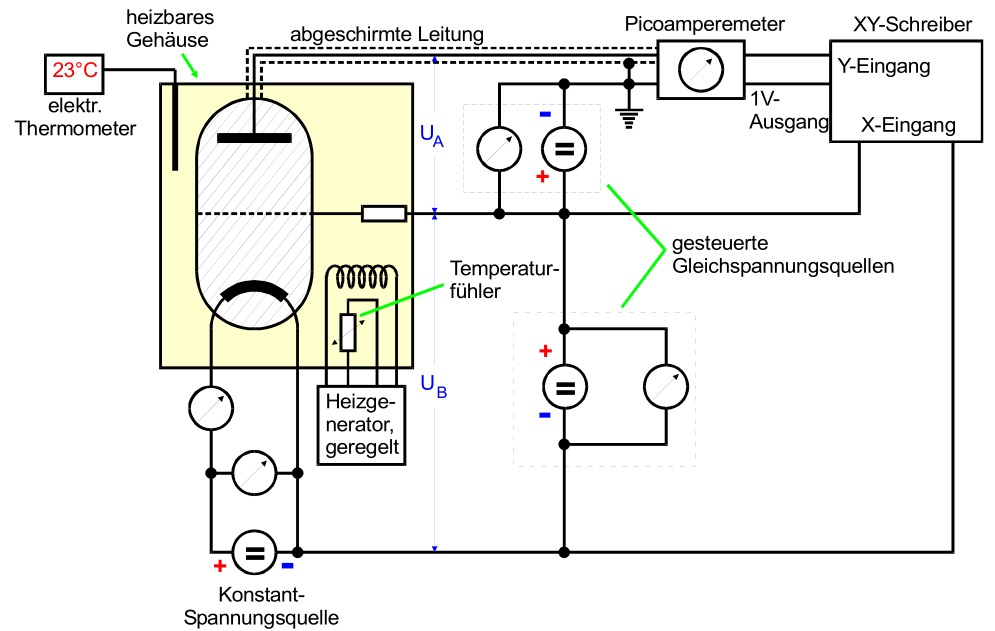
\includegraphics[height=4.0cm]{data/abb3.jpg}
    \caption{Aufbau zur Aufnahme einer Franck-Hertz-Kurve. \cite{V601}}
    \label{fig:abb3}
\end{figure}
Auf dem XY-Schreiber wird das Milimeterpapier befestigt und der Schreiber justiert.
Dazu wird dieser in die untere linke Ecke des Papiers gebracht.
Um den Versuch durchführen zu können werden die einzelnen Elemente wie in der Abbildung \ref{fig:abb3} verkabelt.
Zuerst wird die integrale Enerieverteilung der Elektronen bei verschiedenen Temperaturen T bestimmt.
Wofür die Beschleunigungsspannung $U_B$ auf 11V eingestellt wird.
Bei ausgeschalteter Heizung wird der Auffängerstrom $I_A$ in Abhängigkeit von der Bremsspannung $U_A$ aufgezeichnet.
Danach wird die Heizung eingeschaltet, sodass die nächste Kurve, auf einem neuen Blatt, bei T = (140 - 160) \circ C aufgenommen wird.
Um die Ionisationsenergie von Hg zu bestimmen, wird die Bremsspannung auf −30V eingestellt.
So werden die erzeugten Ionen an der Auffänegrelektrode registriert, die Elektronen aber nicht.
Die Heizung wird so eingestellt, dass diese Messung bei T = (100−110) \circ C stattfindet.
Es wird der Auffängerstrom in Abhängigkeit von der Beschleunigungsspannung aufgetragen.
Die Beschleunigungsspannung wird von 0 bis 60V hochgeregelt.
Die Franck-Hertz-Kurve wird bei einer Temperatur im Bereich von  T = (160 - 200) \circ C aufgenommen.
Die Bremsspannung wird auf -1V eingestellt.